	The experiments were carried out on WZL shop floor, located in Aachen in Germany, acquiring thermal images by means of high speed infrared camera FLIR SC7600 (with framerate of 328 fps and a resoloution of 640 x 512 pixels), it was equipped with a macro lens 1:1 and FOV 9.6 x 7.7 mm. The test bench works in a way that the tool stays in a fixed position in relation to the camera, keeping the relative distance between tool and camera constant, then the scale factor provided by this setting was 15 $\mu$m/pixel. It allows the metric conversion for future post processing of images.

	\begin{figure}[H]
		\centering
		\captionsetup{justification=centering}
		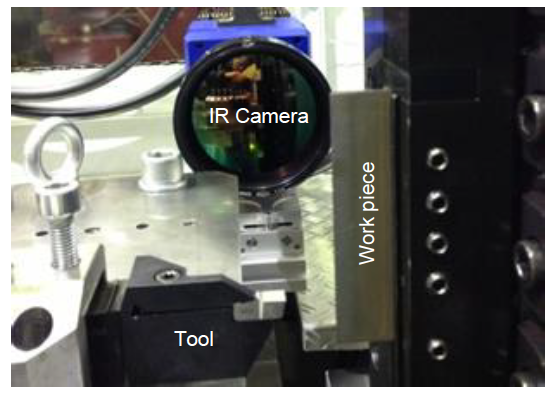
\includegraphics[width=0.9\linewidth]{Cap3/exsetup.png}
		\caption{Experimental setup \cite{augspurger2016experimental}}
		\label{fig:exinfrared}
	\end{figure}

	An important factor for a reliable temperature measurement is the correct choice of the components emissivity. To make it easier, the tool was coated with a black ink, allowing the emissivity valuation for this case, which provided a value of $\epsilon = 0.85$. For the chip case, it was evaluated in its temperature range $\epsilon = 0.4$. It is also important to highlight the camera settings, factors as integration time and filters are essential to determine a reliable measurements due to the amount of eletromagnetic radiation received on camera's sensors. The higher are the temperatures higher is the energy produced, then smaller should be the integration time, which is the time that sensor of energy receives radiation and converts into temperature afterwards. These configurations allowed measurements in a range from 200 $^{o}$C until 900 $^{o}$C.
	
	The tool material was uncoated carbide insert (Sandvik H13A), with rake angle 6$^{o}$, clearance angle 3$^{o}$, cutting radius r$_{\beta}$ < 5$\mu$m and width 4.4 mm. The workpiece material was AISI 1045 normalized and its dimensions were 3.5 x 200 x 80 mm (width, lengh, heigth respectively).
	
	For force acquisition during the process, it was used a three-component piezoelectric force platform, determining the cutting force and passive force. Since the cutting process is carried out in a linear and constant motion, it is possible to determine the overall power $P$ with velocity and cutting force.
	
	All the experiments were were held without coolant, with velocities of 100 $m/min$ and 150 $m/min$ and a$_{p}$ = [0.2, 0.3, 0.4, 0.5] mm.
	The analysis method was built on MATLAB platform with the support of its image processing toolbox. This was the chosen software due the easy connection between FLIR software and MATLAB, since FLIR software can export its images to .mat format, which are indexed matrices prejected to MATLAB environment. Each pixel from the exported images contains information about position and its temperature.

	The design of the experiments are listed on the table bellow:

	\begin{table}[H]
		\centering
		\captionsetup{justification=centering}
		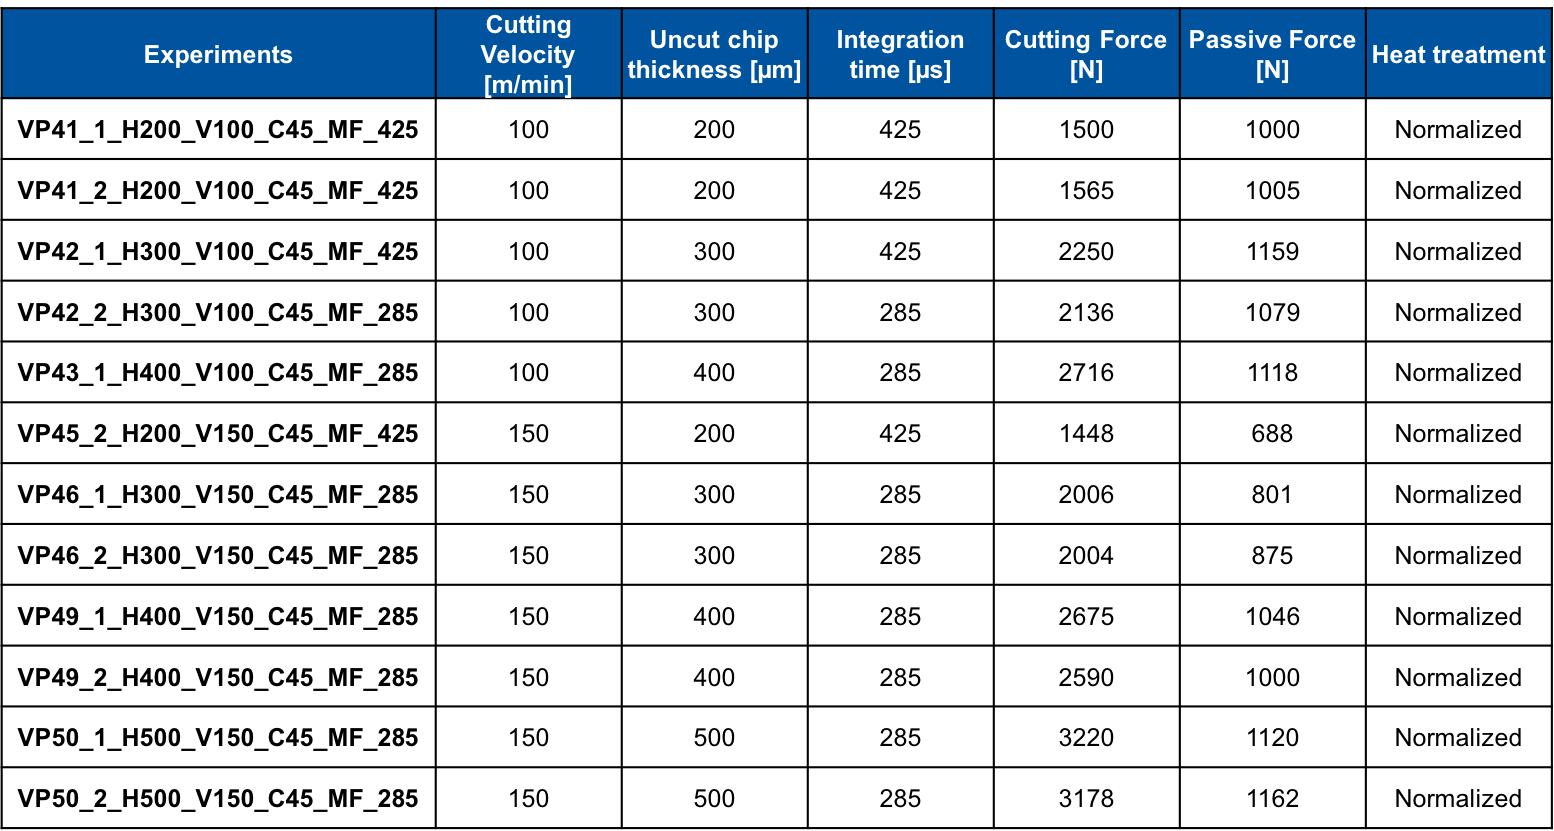
\includegraphics[width=0.9\linewidth]{Cap3/tabexpset.png}
		\caption{Design of experiments \cite{augspurger2016experimental}}
		\label{tab:design}
	\end{table}
 
	% #fazer figura da ferramenta com dimens�es e pe�a tbm
	%fazer figura tool no flir e tool no matlab
	
